\documentclass[
  captions=tableheading,
  bibliography=totoc, 
  titepage=firstiscover,
]{scrartcl}

\usepackage{blindtext} %neuer input

\usepackage{longtable} % Tabellen über mehrere Seiten

\usepackage[utf8]{inputenc} %neuer input

\usepackage{scrhack}

\usepackage[aux]{rerunfilecheck} %Warnung falls nochmal kompiliert werden muss

\usepackage{fontspec} %Fonteinstellungen

\recalctypearea{}

\usepackage[main=ngerman]{babel} %deutsche Spracheinstellung

\usepackage{ragged2e} %neuer input

\usepackage{amsmath, nccmath}

\usepackage{amssymb} %viele mathe Symbole

\usepackage{mathtools} %Erweiterungen für amsmath


\DeclarePairedDelimiter{\abs}{\lvert}{\rvert}
\DeclarePairedDelimiter{\norm}{\lVert}{\rVert}

\DeclarePairedDelimiter{\bra}{\langle}{\rvert}
\DeclarePairedDelimiter{\ket}{\lvert}{\rangle}

\DeclarePairedDelimiterX{\braket}[2]{\langle}{\rangle}{
#1 \delimsize| #2
}

\NewDocumentCommand \dif {m}
{
\mathinner{\symup{d} #1}
}


\usepackage[
  math-style=ISO,
  bold-style=ISO,
  sans-style=italic,
  nabla=upright,
  partial=upright,
  warnings-off={
    mathtools-colon,
    mathtools-overbracket,
  },
]{unicode-math}

\setmathfont{Latin Modern Math}
\setmathfont{XITS Math}[range={scr, bfscr}]
\setmathfont{XITS Math}[range={cal, bfcal}, StylisticSet=1]


\usepackage[
  locale=DE,
  separate-uncertainty=true,
  per-mode=reciprocal,
  output-decimal-marker={,},
]{siunitx}

\usepackage[autostyle]{csquotes} %richtige Anführungszeichen

\usepackage{xfrac}

\usepackage{float}

\floatplacement{figure}{htbp}

\floatplacement{table}{htbp}

\usepackage[ %floats innerhalb einer section halten
  section,   %floats innerhalb er section halten
  below,     %unterhalb der Section aber auf der selben Seite ist ok
]{placeins}

\usepackage[
  labelfont=bf,
  font=small,
  width=0.9\textwidth,
]{caption}

\usepackage{subcaption} %subfigure, subtable, subref

\usepackage{graphicx}

\usepackage{grffile}

\usepackage{booktabs}

\usepackage{microtype} %Verbesserungen am Schriftbild

\usepackage[
backend=biber,
]{biblatex}

\addbibresource{../lit.bib}

\usepackage[ %Hyperlinks im Dokument
  german,
  unicode,
  pdfusetitle,
  pdfcreator={},
  pdfproducer={},
]{hyperref}

\usepackage{bookmark}

\usepackage[shortcuts]{extdash}

%\usepackage{warpcol}


\begin{document}
    \title{ATP Übungsblatt 6}
    \author{  
    Tobias Rücker\\
    \texorpdfstring{\href{mailto:tobias.ruecker@tu-dortmund.de}{tobias.ruecker@tu-dortmund.de}
    \and}{,} 
    Paul Störbrock\\
    \texorpdfstring{\href{mailto:paul.stoerbrock@tu-dortmund.de}{paul.stoerbrock@tu-dortmund.de}}{}
    }
\maketitle
\center{\Large Abgabegruppe: \textbf{Mittw. 10-12 Uhr}}
\thispagestyle{empty}

\newpage
\tableofcontents
\thispagestyle{empty}
\newpage

\setcounter{page}{1}

\section{Aufgabe 16}

    \begin{figure}[H]
        \centering
        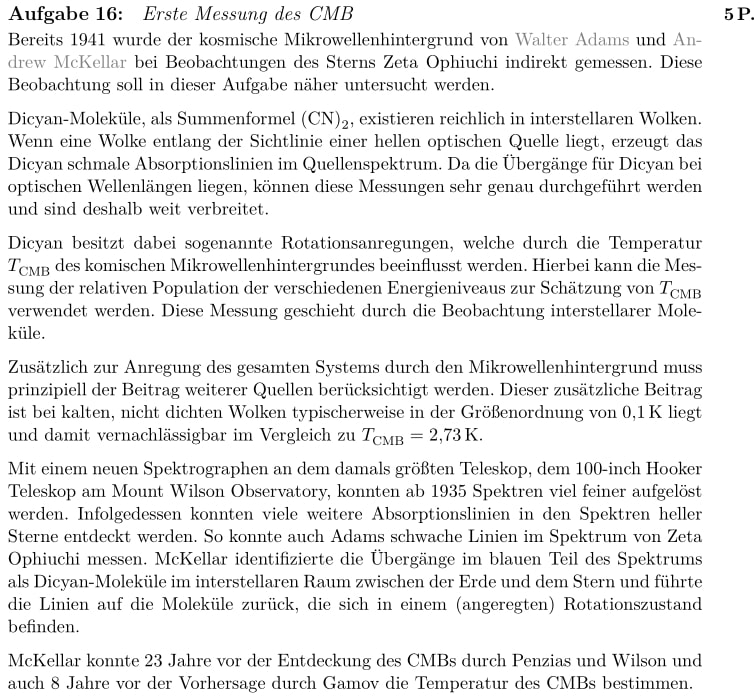
\includegraphics[width=\textwidth]{images/Aufgabe16a.jpg}
        \label{fig:1}
    \end{figure}

    \begin{figure}[H]
        \centering
        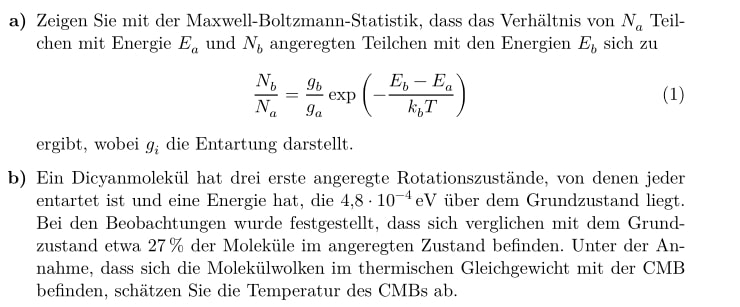
\includegraphics[width=\textwidth]{images/Aufgabe16b.jpg}
        \label{fig:2}
    \end{figure}

\subsection{a)}
Nach der Maxwell-Boltzmann Statistik ergibt sich für die Anzahl der Teilchen
\begin{align}
    \frac{\langle N_i \rangle }{N} &= \frac{1}{Z} \frac{g_i}{e^{-\frac{E_i}{k_b T}}}\\
    \langle N_i \rangle &= \frac{N}{Z} \frac{g_i}{e^{-\frac{E_i}{k_b T}}}\\
    \frac{\langle N_b \rangle}{\langle N_a \rangle} &= \frac{g_b}{g_a} e^{\frac {-E_b+E_a}{k_b T}}\\
    \frac{\langle N_b \rangle}{\langle N_a \rangle} &= \frac{g_b}{g_a} e^{-\frac {E_b+E_a}{k_b T}}
\end{align}

\subsection{b)}
\begin{align}
    \ln \left(\frac{N_b}{N_a} \frac{g_a}{g_b} \right) &=- \frac{E_b-E_a}{k_b T}\\
    T&= -\frac{E_b-E_a}{k_b \ln \left(\frac{N_b}{N_a} \frac{g_a}{g_b} \right)}
    \intertext{
        27\% der Moleküle im angeregten Zustand
    }
    \Rightarrow \frac{N_b}{N_a}=0,27
    \intertext{
        angeregter Zustand ist um $\SI{4.8e-04}{\electronvolt} $
    }
    \Rightarrow E_b &= E_a +\SI{4.8e-04}{\electronvolt}
    \intertext{
        $g_a=1$ und $g_b =3$
    }
    T &= - \frac{\SI{4.8e-04}{\electronvolt}}{k_b \ln \left(0,27 \frac{1}{3} \right) }\\
    T &= \SI{2.313}{\kelvin}
\end{align}


\section{Aufgabe 17}

    \begin{figure}[H]
        \centering
        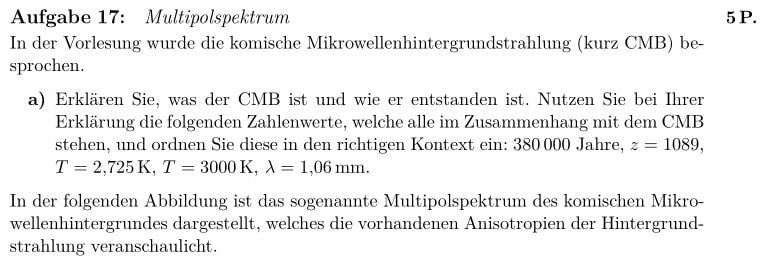
\includegraphics[width=\textwidth]{images/Aufgabe17a.jpg}
        \label{fig:3}
    \end{figure}

    \begin{figure}[H]
        \centering
        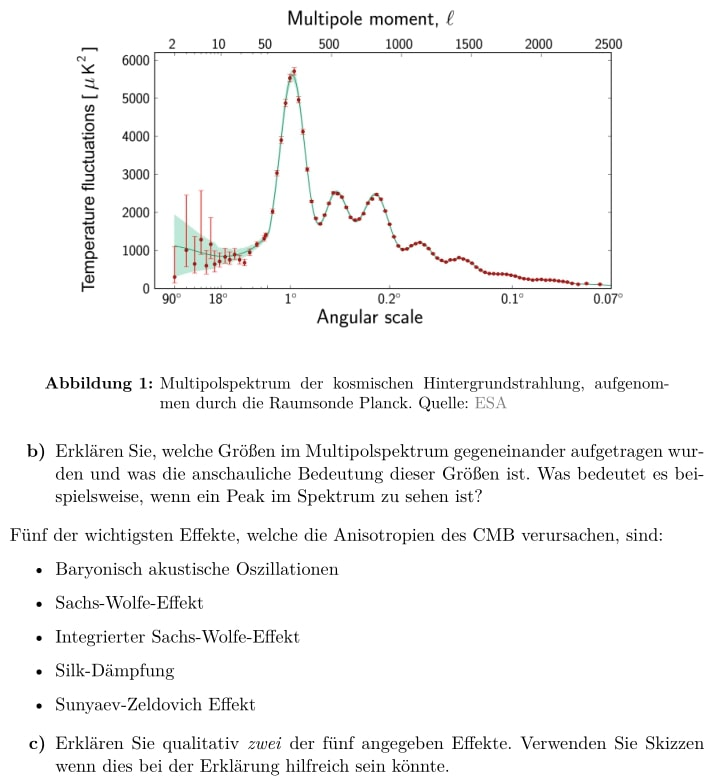
\includegraphics[width=\textwidth]{images/Aufgabe17b.jpg}
        \label{fig:4}
    \end{figure}

\subsection{a)}

    \flushleft{Als\;}\justifying cosmic microwave background (CMB) wird die elektromagnetische Strahlung bezeichnet, die wir auf der Erde messen können, die aber nicht von der Erde stammt. 
    Der CMB entstand im frühen Universum, wo das Universum aus einer Dichten Masse (Plasma) bestand, welche wiederum aus Protonen und Elekronen bestand. Über einen Zeitraum von 380000 Jahren
    hat sich diese Masse soweit ausgedehnt, dass sich die Protonen und Elekronen zu Wasserstoff Kernen fusionieren konnten. Dies geschah bei einer Temperatur von ca. 
    \SI{3000}{\kelvin}. Da elektromagnetische Strahlung von der Lorenzkraft beinflusst wird, hatte die Rekombination der Protonen und Elekronen die Freisetzung jener Strahlung zur Folge.
    Denn die entstandenen Neutronen und Photonen wechselwirken nicht miteinander, was es dem Licht erlaubt der abgekühlten Plasmawolke zu entkommen. Nun sind Materie und Strahlung nicht
    mehr gebündelt. Dieser Zeitpunkt wird auch als surface of last scattering bezeichnet, welcher für den heute zu messenden CMB verantwortlich ist. Durch die Expansion des Raums 
    wurden die freigesetzten Photonen um einen Faktor von $z=$ 1089 gestreckt, was einer besonders starken Rotverschiebung zugrunde liegt. Durch die Rotverschiebung scheit die Temperatur der emittierten Photonen
    deshalb gleich der eines Schwarzkörpers von \SI{2.725}{\kelvin} zu sein. Wird also das Leistungsspektrum der Strahlung $\sfrac{\partial E(\lambda)}{\partial \lambda}$ gegen die Wellenlänge
    $\lambda$ aufgetragen, ergibt sich aus der enstehenden Kurve das Maximum der Wellenlänge $\lambda=$ \SI{1.06}{\milli\meter}. Die Kurve zeigt, dass das Licht trotz einer relativ homogenen
    Emission unterschiedlich stark gestreckt wurde. 

\subsection{b)}

    \flushleft{Baryonisch\;}\justifying akustische Oszillationen:\\
    Baryons beschreibt Materie wie Neutronen und Protonen, welche aus drei Quarks bestehen. Diese waren die Bausteine des frühen Universums, vor dem Zeitpunkt des surface of last scattering.
    Die akustischen Oszillationen enstanden dadurch, dass  

\subsection{c)}





\section{Aufgabe 18}

    \begin{figure}[H]
        \centering
        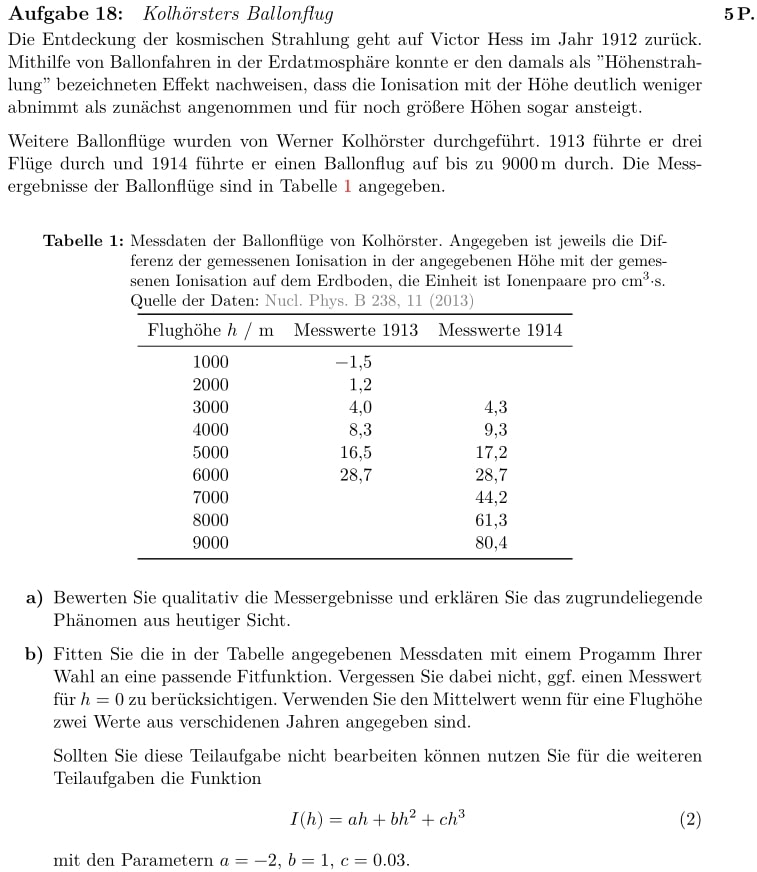
\includegraphics[width=\textwidth]{images/Aufgabe18a.jpg}
        \label{fig:5}
    \end{figure}

    \begin{figure}[H]
        \centering
        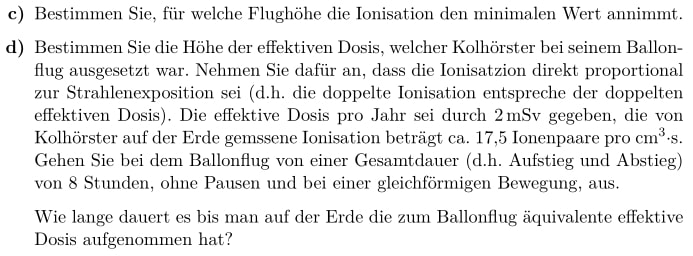
\includegraphics[width=\textwidth]{images/Aufgabe18b.jpg}
        \label{fig:6}
    \end{figure}

\subsection{a)}

    \flushleft{Vor\;}\justifying Kohlhörsters Experiment, wurde angenommen, dass der Strahlungshintergrund ausschließlich von der Untergrundstrahlung der Erde ausgeht. 
    Demnach sollte der Strahlungshintergrund mit zunehmender Höhe abfallen. Kohlhörsters Ballonflug hingegen zeigte, dass die nicht der Fall ist. Sondern vielmehr, dass
    der Strahlungshintergrund bei zunehmender Höhe auf ein Vielfaches dessen steigt, was am Erdboden gemessen wird. Interessanterweise, wird bei einer relativ geringen 
    Höhe (ca.1000m) ein Abfall der Strahlung gemessen, was mit der vorherigen Ansicht, nämlich, dass die Untergrundstrahlung bei zunehmender Höhe abnimmt, übereinstimmt.\\
    Heutzutage wissen wir, dass die gemessene kosmische Strahlung bei größerer Höhe immer weiter zunimmt. Dies hat mit der Ionisation der Luft zu tun, die bei zunehmender
    Höhe an Dichte verliert, weshalb die kosmische Strahlung weniger abgeschiermt werden kann.

\subsection{b)}

    \flushleft{Die\;}\justifying folgende Tabelle gibt die Mittelwerte der in den Jahren 1913 und 1914 gemessenen Strahlungsintensitäten und die dazugehörige Höhe wieder. 

    \begin{table}[H]
        \centering
        \caption{Höhe gegen Mittelwerte der Messwerte aus 1913 und 1914}
        \input{build/table18.tex}
        \label{tab:1}
    \end{table}

    \flushleft{Mithilfe\;}\justifying der Messwerte aus Tabelle \ref{tab:1}, der Gleichung:
    \begin{align*}
        I(h) &= ah+bh^2+ch^3\\
        \intertext{
            \flushleft{und\;}\justifying den dazugehörigen Parametern
        }
        a &= \text{\input{a.tex}}\\
        b &= \phantom{-}\text{\input{b.tex}}\\
        c &= \phantom{-}\text{\input{c.tex}}
        \intertext{
            \flushleft{lässt\;}\justifying sich der folgende Graph erstellen:
        }
    \end{align*}

    \begin{figure}[H]
        \centering
        \includegraphics[width=\textwidth]{build/plot18.pdf}
        \label{fig:7}
    \end{figure}

\subsection{c)}

    \flushleft{Das\;}\justifying Ionisationsminimum liegt bei:
    \begin{align*}
        h_{min} &= \text{\input{h_min.tex}}
    \end{align*}

\subsection{d)}





\end{document}